\section{Exploratory data analysis}

\subsection{Principal component analysis }

To further explore patterns in the data, a Principal Component Analysis (PCA) was performed by singular value decomposition on the meteorite data.
Because PCA is very sensitive to outliers some procedures had to be performed on the data in advance of the svd. First,
the data was centered by pertubing with the geomtric mean. Next, the data was scaled by the inverse square 
root of the total variance, normalizing its overall dispersion to prevent domination by highly variable components Finally, 
the data was CLR-transformed; this step ensures that the Euclidean distance metric implied in the SVD is valid for our data.  

The PCA has been visualised using a biplot and screeplot in Fig. \ref{fig:pcabiplot}. The biplot shows the first two principal components of the data with the samples
represented as points/samples and the variables/parts as arrows. The length of the arrow indicates the importance of the variable in the PCA, and the angle between the arrows indicates how correlated they are.
The screeplot shows the proportion of variance explained by each principal component, which is useful for determining how many components to retain in the analysis. 

In this case, the scree plot shows that with only two components, we can explain 96\% of the variance in the dataset, indicating that this decomposition is highly useful for further analysis.

At first glance of the biplot we see that all the loadings of the metal oxides tend point in the same direction, this means that they are all positively correlated, while the pure metals \{Ni, Co, Fe\} is opositely correlated as the loadings of these metals points in the oposite direction of loadings of the metal oxides. This means that when we see a lot of metaloxides in a meteorite we will not see a lot of the pure metals and vice verse. The loading of Carbon on the other hand is somewhat 
perpedicular to the rest of the loadings, which suggests that there is neither a strong nor negative correlation between the 
C and the rest of the metals. 



\begin{figure}[htbp]
    \centering
    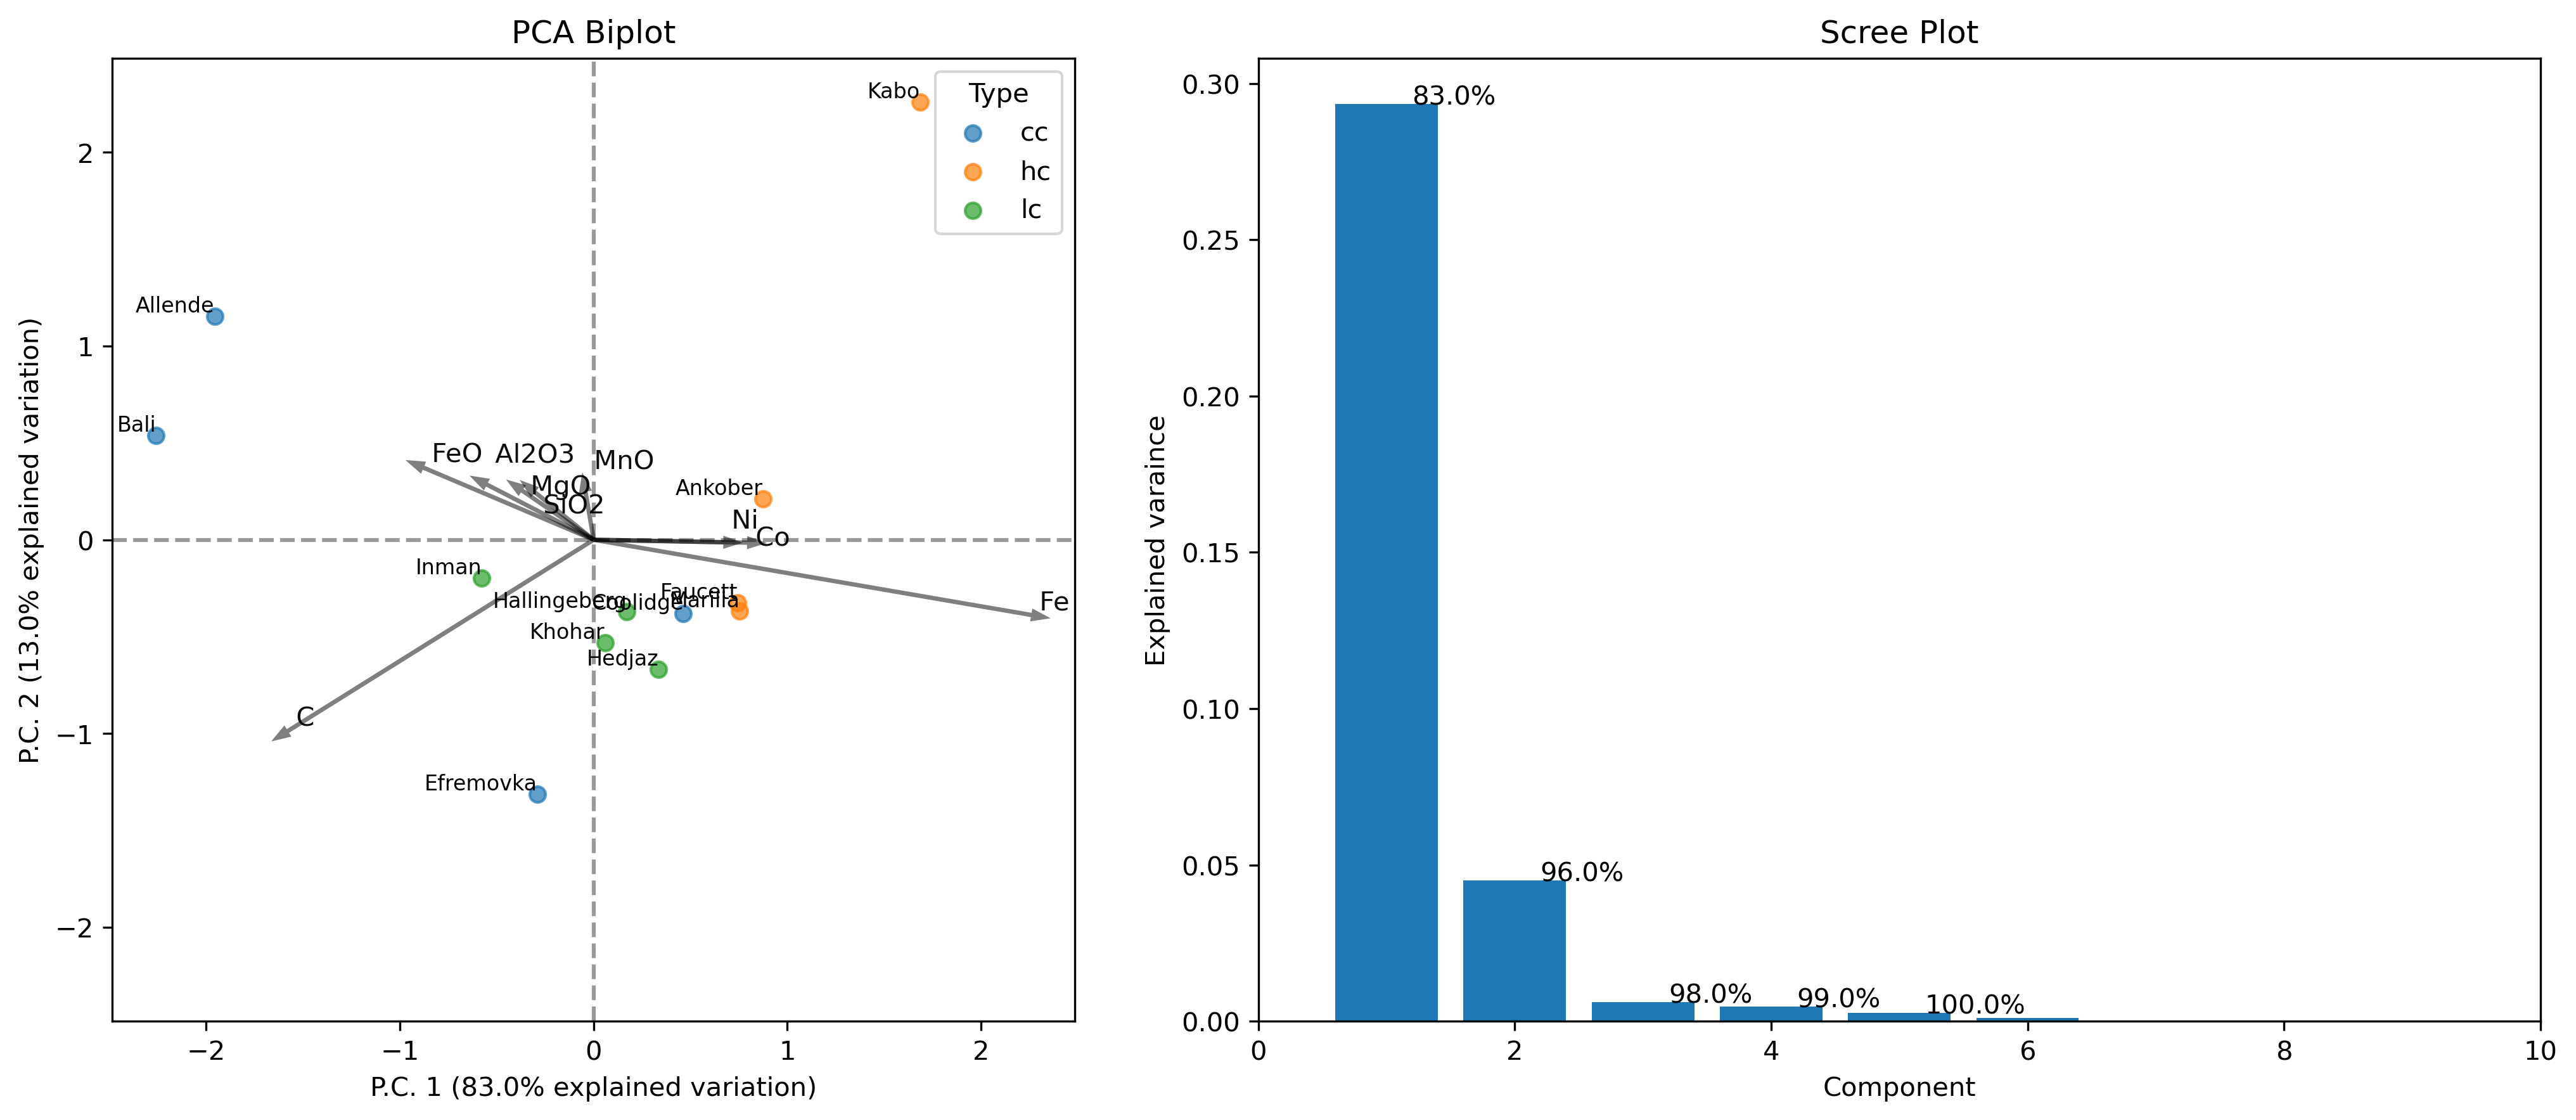
\includegraphics[width=0.8\textwidth]{figures/pca_biplot.png}
    \caption{Example plot showing the chemical composition of meteorites.}
    \label{fig:myplot}
\end{figure}
 %

\subsection{Subcompositional analysis }

From the Fig. \ref{fig:pcabiplot}, we can identify a few subcompostions where two parts loadings vertices 
are allined, the most profound of these being Carbon perpandicular to 

